\chapter{Diseño del Algoritmo Genético Propuesto ArcGen}\label{cap3}

\section{Algoritmo para Grafos Completos}
	%permite una representación del grafo de tal manera que los cruces que se obtenga de los nodos sean causa del orden de los nodos en una línea, y de la dirección (superior o inferior) que se le da al arco al dibujarlo, como puede observarse
	Debido  a la  simplicidad de los Arc Diagram para esquematizar a los  grafos,  es que se  utiliza esta representación en busca de un grafo con una mínima cantidad de cruces de arcos.
	
	Así, se desarrolla  un algoritmo que permite visualizar  grafos  completos, es decir, aquellos donde cada par de vértices está conectado por un arco, como un Diagrama de Arcos y que  soluciona el Crossing Number.
	%Inicialmente,  se plantea un método de ordenamiento que permita solucionar el Crossing Number para grafos completos, es decir, donde todos sus nodos están conectados con arcos a los restantes nodos. 
    Dado que el  grafo es completo, todos  los vértices tienen la misma cantidad de arcos,  luego se considera que todos los nodos poseen el mismo peso o importancia en el grafo. %Esto  no es posible ponderar a los nodos. no se diferencian de los demás.

	
	%figura mostrando K6 no óptimo
	
	A partir de un grafo completo se  genera  el  Diagrama de Arcos correspondiente, con  el mejor ordenamiento tanto de posición de los nodos sobre la línea, como de la ubicación de los arcos en el  plano,  tal que el número de cruces de arcos sea minimal.
	
	A fin de lograr esta representación óptima de cruces, no es necesario tener en cuenta el orden de los nodos, ya que, todos disponen de la misma cantidad de arcos salientes. Por lo tanto, el algoritmo se centra en distribuir los arcos de manera que su disposición sea equitativa, tanto en el semiplano  superior como en el inferior.
	
	La distribución de arcos se realiza comenzando por  dibujar  todos los arcos de los nodos de los extremos de la  recta, iniciando por la izquierda. Aquellos del nodo en el extremo  izquierdo  se dibujan en el semiplano  superior y aquellos del  nodo en el extremo  derecho en el inferior. Luego se continua dibujando los arcos correspondientes a los  nodos inmediatos al  procesado anteriormente en sentido al  centro de la línea, esquematizando primero el del lado izquierdo y luego el derecho. En la Figura \ref{fig:arcdiagram_k6_no_optimo}\ se muestra como  se visualiza  un grafo completo de 6 nodos.
	
	\begin{figure}[h]
		\centering
		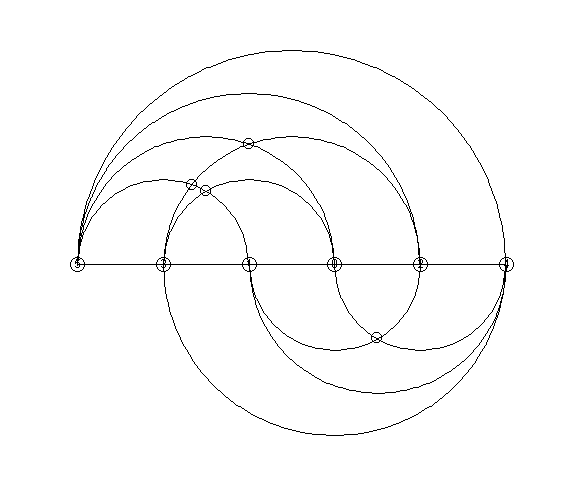
\includegraphics[width=8cm]{imagenes/grafo_1_bn.png}
		\caption{Diagrama de Arcos de un grafo completo de 6 nodos ($K_6$).}
		\label{fig:arcdiagram_k6_no_optimo}
	\end{figure}
	
	La  visualización  del grafo resultante de aplicar el algoritmo no resulta óptimo en cuanto a cantidad de cruces. Esto es posible de verificar debido a la conjetura que  plantea Guy en \cite{guy1960combinatorial},  que  da una cota superior para calcular el Crossing Number de grafos completos, notado $cr$,  y que proporciona un punto de referencia para medir la efectividad de nuestro algoritmo.
	
	$$cr(K_n) \leq \frac{1}{4} \floor*{\frac{n}{2}} \floor*{\frac{n-1}{2}} \floor*{\frac{n-2}{2}} \floor*{\frac{n-3}{2}}$$
	En nuestro  ejemplo, $cr(K_6)=3$ pero el dibujo del grafo  tiene 4 cruces.
	
	%A fin de resolver este problema, se buscaron los arcos que presentaban el problema, en grafos con diferentes cantidades de nodos. 
	
	A partir de la visualización de  una serie de grafos completos, se logra descubrir  que la aparición de cruces conflictivos  siguen un  patrón. En la Figura \ref{fig:arcdiagram_no_optimo} se presenta el patrón de los  arcos  conflictivos sobre cuatro grafos completos. 
	
	%podemos visualizar tal patrón, donde según el total de nodos podemos ver que se presentan más arcos conflictivos en lados opuestos, los cuales al invertirlos de sentido permiten eliminar los cruzamientos extras.
	
	\begin{figure*}[h]
		\centering
		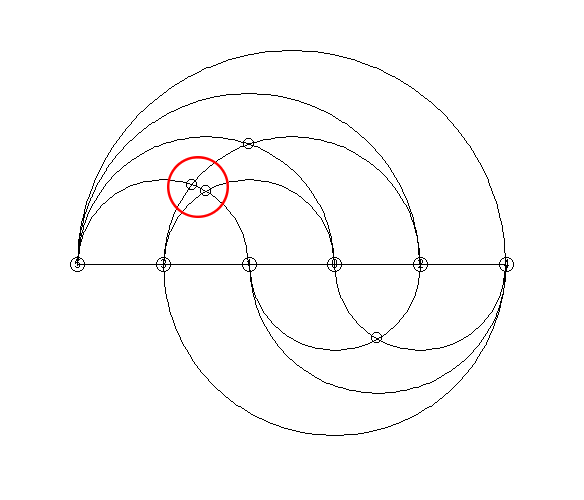
\includegraphics[width=5cm]{imagenes/grafo_1_bn_no_opt.png}
		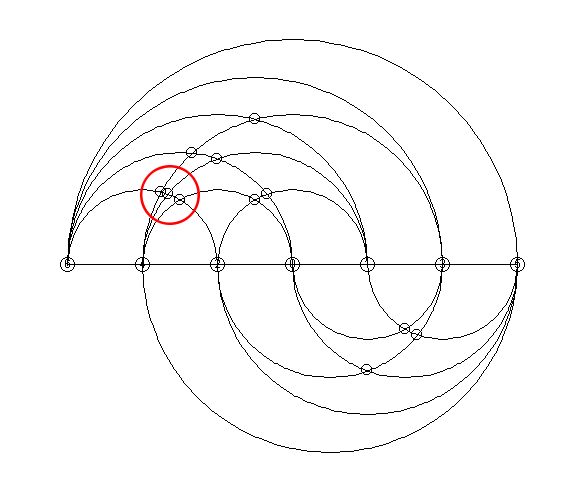
\includegraphics[width=5cm]{imagenes/grafo_2_bn_no_opt.png}\\
		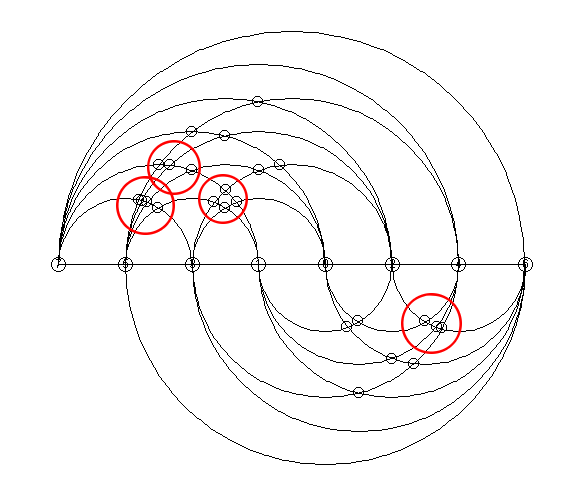
\includegraphics[width=5cm]{imagenes/grafo_3_bn_no_opt.png}
		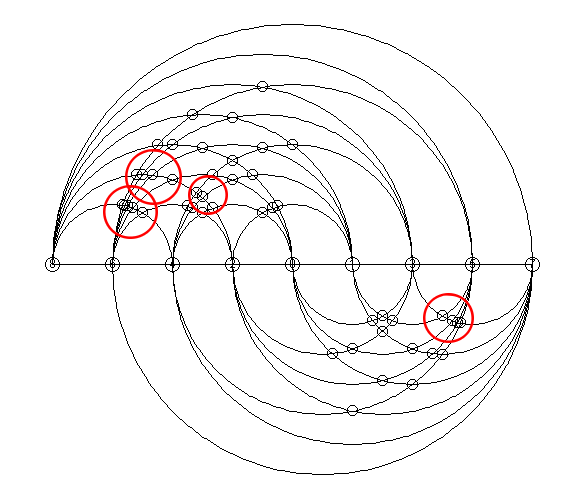
\includegraphics[width=5cm]{imagenes/grafo_4_bn_no_opt.png}
		\caption{Diagrama de Arcos de grafos completos $K_6$, $K_7$, $K_8$ y $K_9$ donde se puede visualizar cruces que siguen un patrón.}
		\label{fig:arcdiagram_no_optimo}
	\end{figure*}
	
	%figura mostrando K6,K7,K8,K9 sin optimización
	
	Así, para solucionar el problema, se plantea una serie de transposiciones de arcos, cambiando el semiplano en donde está dibujado. El  número de transposiciones se determina según el patrón que siguen los grafos y  se calcula a partir de la cantidad de nodos, como:	$$t(n) = \floor*{\frac{n}{2}}-2,\ \mbox{con } n\geq 5.$$
	
	El algoritmo hace un recorrido sobre $t(n)$ nodos en la recta igual al de la distribución de los arcos en los semiplanos, comenzando en los extremos, esto es $nodo_1, nodo_n, nodo_2, nodo_{n-1}, \ldots, nodo_{n / 2}$. Para cada uno de los $t(n)$ nodos que recorre, se transponen $t(n), t(n)-1, t(n)-2, \ldots, 1$ arcos,  cambiando el  semiplano donde se dibujan, siempre que no aumente el número de cruces. Para el nodo actual $n_a$, los arcos a transponer se seleccionan ordenados por la cercanía que hay entre  $n_a$ y el nodo en el otro extremo del arco, sin tener en cuenta el  arco que une a  $n_a$ con el siguiente en la recta.
	%a la generación de  transpone primero los $t(n)$ arcos conectados al nodo más próximo hacia el centro del grafo por el lado izquierdo, sin contar el nodo central (cuando $n$ es impar). Luego se saltea hacia el nodo en el extremo derecho y se reduce a  $t(n)-1$ siempre que sea positivo,  la cantidad de cambios, nuevamente invirtiendo desde el nodo mas próximo sin contar el primero. El proceso se repite con el nodo próximo al nodo del extremo izquierdo, y luego al próximo del extremo derecho y así sucesivamente, 
	En la Figura \ref{fig:arcdiagram_optimo}, se muestra el resultado de la  aplicación del proceso de  transposición.
	
	%	\todo[inline]{VER si lo ponemos: Este proceso se ha probado con grafos de más nodos, y se encontró en algunos casos que el cambio producía más cruces que los indicados por $cr(K_n)$ según la conjetura. Para solucionar esto se consideró evaluar los cruces de arcos antes y después de cambiar el arco de semiplano, y quedándose con el grafo que disponga menos. De esta manera el número $t(n)$ ya no determina la cantidad exacta de transposiciones de arcos sino que corresponde con una cota superior de transposiciones necesarias para la optimización.}
	
	\begin{figure*}[h]
		\centering
		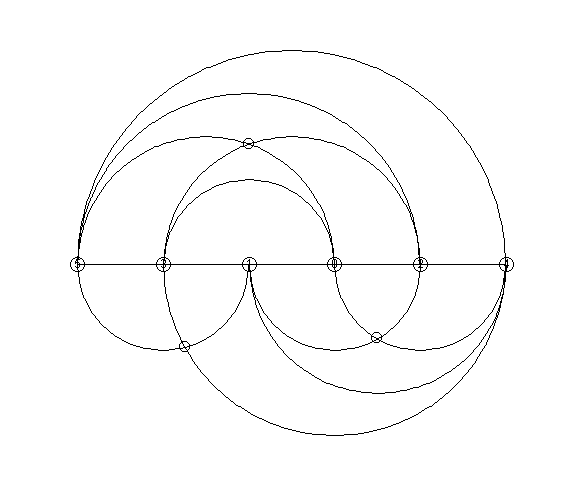
\includegraphics[width=5cm]{imagenes/grafo_1_bn_opt.png}
		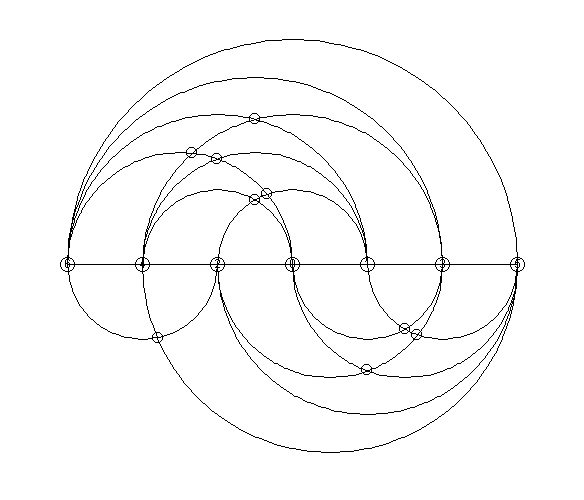
\includegraphics[width=5cm]{imagenes/grafo_2_bn_opt.png}\\
		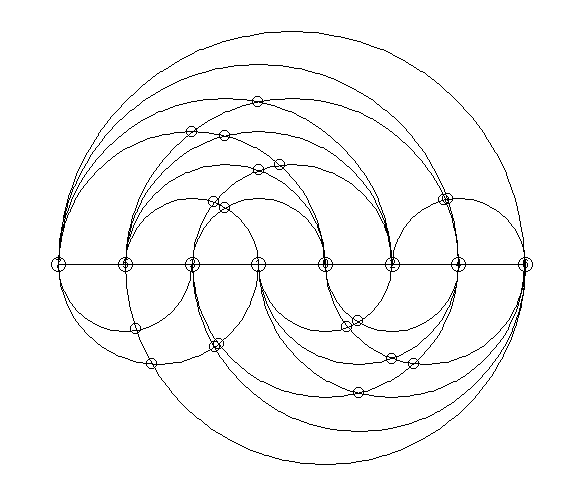
\includegraphics[width=5cm]{imagenes/grafo_3_bn_opt.png}
		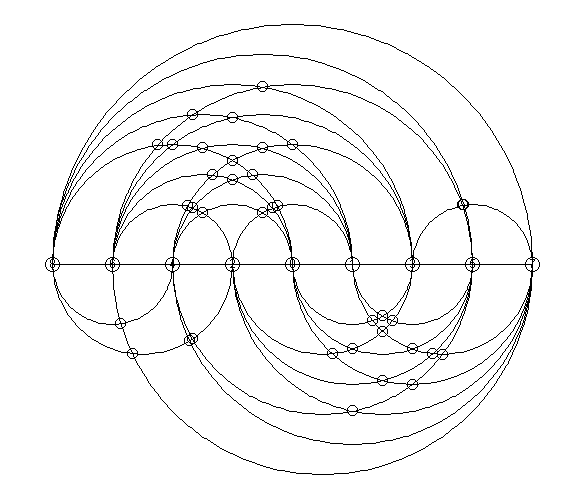
\includegraphics[width=5cm]{imagenes/grafo_4_bn_opt.png}
		\caption{Diagrama de Arcos de grafos completos $K_6$, $K_7$, $K_8$ y $K_9$ luego de solucionar los conflictos advertidos en la Figura \ref{fig:arcdiagram_no_optimo}.}
		\label{fig:arcdiagram_optimo}
	\end{figure*}
	
	%figura mostrando K6,K7,K8,K9 con optimización
	
	Esta optimización nos permite obtener  una representación gráfica de un grafo completo con el mínimo Crossing Number, comparado con la conjetura dada. En forma empírica esta suposición ha sido probada hasta $K_{100}$.
	
	
	A partir de esto se propone utilizar el algoritmo para un  grafo arbitrario, buscando que su Crossing Number sea minimal. Al permitir que los nodos puedan variar en cantidad de arcos, el algoritmo también debe tener en cuenta el orden de los mismos en la línea de nodos. A fin de  determinar un peso relativo para los nodos, dando un valor a partir del cuál se pueda proponer un orden para los nodos que obtenga un Crossing Number  mínimo o lo más bajo en lo posible, se introducen dos conceptos.
	
	%\begin{definition}[Grado de Nodo]
	%		El grado de un nodo se define como la cantidad de arcos que conectan con él.
	%	\end{definition}
	
	\begin{definition}[Grado de Arco]
		El grado de un arco se define como el grado más alto de los dos nodos que conecta, siendo el grado de un nodo la cantidad de arcos que conectan con él.
	\end{definition}
	
	El grado de arco permite dar una ponderación a cada arco según los nodos que conecta. De este  modo, se obtiene una cota superior en la cantidad de  nodos alcanzables desde los  extremos del arco.
	
	\begin{definition}[Nivel de Nodo]
		El nivel de un nodo se define como el grado más bajo de los arcos que conectan con él.
	\end{definition}
	
	%Definiciones formales de grado  de arco y nivel del nodo y ejemplos de estas definiciones.
	
	%Reordenamiento de  los nodos según el nivel del nodo.\\
	
	Intuitivamente,  el Nivel de Nodo permite determinar el  peso que tiene el nodo en el grafo, según sus relaciones con los demás nodos y así, da un criterio para ordenar los nodos del grafo en la recta,  antes de trazar los arcos. Un nodo con mayor conectividad se considera de mayor interés al  dibujar el grafo. %más interesante en un grafo, pero también es importante tener en cuenta el peso de las conexiones o arcos en sí mismas, para lo cuál se plantea el Grado de Arco, que surge del Grado de Nodo de los dos nodos que conecta. Este último se determina según la cantidad de arcos que salen de él, y permite al anterior dar una ponderación a cada arco según los nodos que conecta. Finalmente se define el nivel de nodo basado en los grados de sus arcos, para poder dar un peso al nodo con respecto a sus relaciones y al peso de las mismas.
	
	Dado el nivel de nodo se realiza un ordenamiento de los mismos de manera que aquellos con mayor nivel permanezcan lo más alejados posible entre ellos en la recta, buscando que se produzcan, de esta manera, la menor cantidad de cruzamientos entre sus arcos. Para ello se ubican en la recta los nodos en orden decreciente de nivel, ordenándolos en extremos opuestos del grafo de manera que queden lo más alejados del nodo anterior de mayor nivel y dejando aquellos de menor nivel en el centro del grafo, como se muestra en la Figura \ref{fig:arcdiagram_no_completo}.
	
	\begin{figure*}[h]
		\centering
		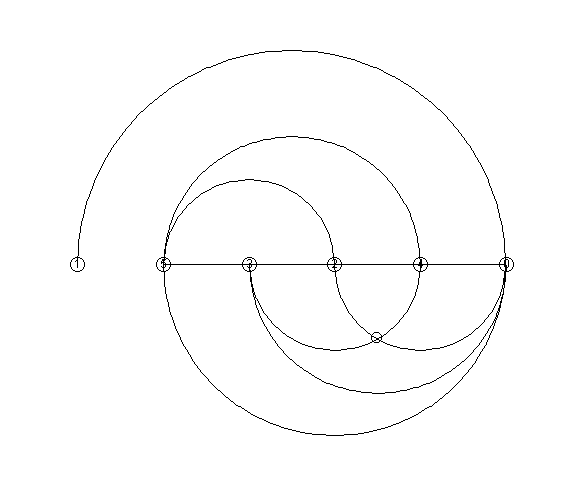
\includegraphics[width=5cm]{imagenes/grafo_aleatorio_6_nodos_bn.png}
		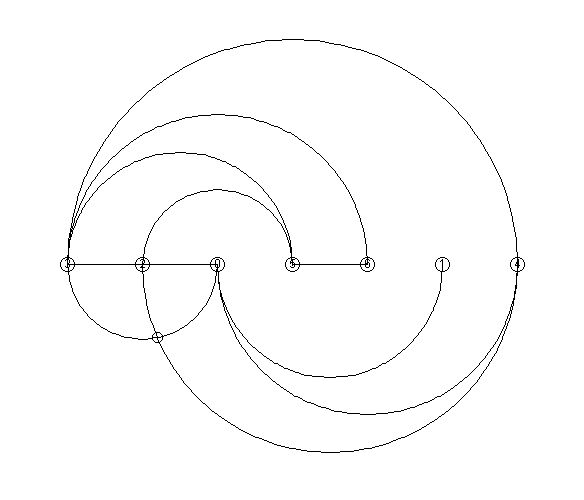
\includegraphics[width=5cm]{imagenes/grafo_aleatorio_7_nodos_bn.png}\\
		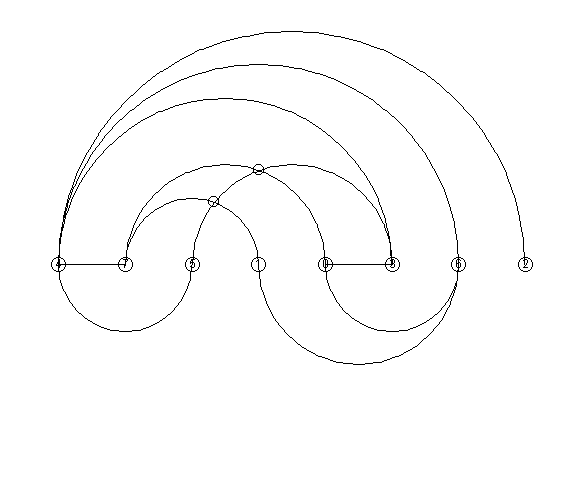
\includegraphics[width=5cm]{imagenes/grafo_aleatorio_8_nodos_bn.png}
		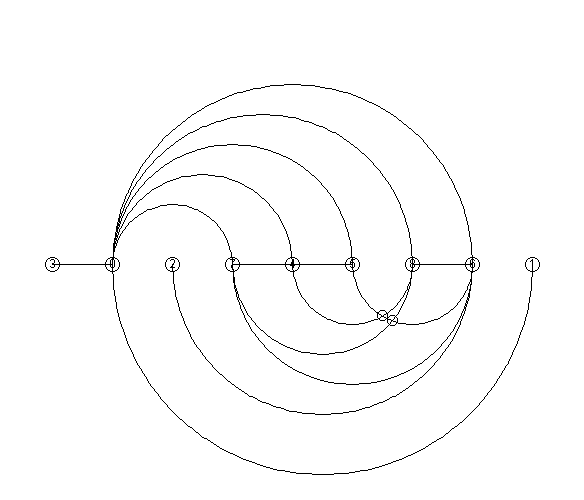
\includegraphics[width=5cm]{imagenes/grafo_aleatorio_9_nodos_bn.png}
		\caption{Diagrama de Arcos de grafos no completos generados aleatoriamente, en los cuáles se aplicó el algoritmo para Crossing Number mínimo en grafos completos.}
		\label{fig:arcdiagram_no_completo}
	\end{figure*}
	
	%figura de ejemplo de Diagrama de Arcos no completo utilizando algoritmo optimo para completo
	
	Este criterio de ordenamiento junto con el algoritmo presentado anteriormente  para trazar los arcos, permiten obtener un Diagrama de Arcos con relativamente pocos cruces, pero que  no es óptimo  como lo era en grafos completos. Ya que los grafos no completos  no respetan el patrón de arcos en conflicto descubierto para los grafos completos, 
	no es posible aplicar la optimización descripta anteriormente.
	
	En conclusión, los algoritmos presentados  permiten  obtener un Diagrama de Arcos óptimo con respecto al Crossing Number en grafos completos, probado empíricamente hasta $K_{100}$, y relativamente bueno con respecto a grafos no completos. Esta visualización rectilínea de los grafos es el  punto de partida del algoritmo  que presentaremos en la siguiente sección para minimizar la cantidad de cruzamiento de arcos. 
	%para llegar a un resultado más satisfactorio con respecto a los cruzamientos de arcos y así acercarnos más a una mejor visualización, lo cuál es la finalidad de este trabajo.
	
	%Aplicación del algoritmo que devuelve un arc graph relativamente óptimo para  grafos completos con menor crossing
	%Un algoritmo  que permite que un grafo completo obtenga la menor cantidad de cruces,  hace que un grafo cualquiera tenga pocos cruces.

\section{Algoritmo ArcGen}

%	En la sección anterior hemos obtenido un Diagrama de Arcos, que a partir de un algoritmo sencillo y eficiente permite obtener un Crossing Number óptimo para arcos completos y uno relativamente bueno para grafos no completos. Ahora buscaremos optimizar estos últimos de manera que se pueda conseguir un resultado más satisfactorio, pero considerando algunas limitaciones en los grafos que trabajaremos.
	
	Motivados por una adecuada visualización de  modelos conceptuales, se diseñó e implementó  un nuevo algoritmo genético, considerando algunas limitaciones sobre los grafos que esquematizan estos diagramas, como el  hecho de que 
	%y diagramas de dominio que por lo general
	generalmente disponen de  grandes cantidades de entidades o clases (nodos del grafo), aunque disponen de cantidades moderadas o pequeñas de relaciones (arcos del grafo).
	El  algoritmo genético propuesto  mejora los resultados obtenidos con el algoritmo presentado en la sección anterior, que representa al grafo  con un Diagrama de Arcos. De hecho, este último se utiliza como un preprocesamiento sobre el grafo original,  para la generación de la población inicial del algoritmo genético.  Esto permite evolucionar  hacia  un grafo  con menos cruces (mínimo local) o  hacia el óptimo (mínimo número de cruces)  con  relativamente pocos cambios sobre el Diagrama de Arcos, y por lo tanto, obtener el resultado en  pocas generaciones. %Pero siempre buscando acotar el problema al objetivo que se planteó.
	
	\subsection{Representación de  los Individuos}
	\label{subsec:representacion_individuos}
	Cada individuo de la población corresponde a un Diagrama de Arcos. La representación incluye  los nodos y arcos del grafo, el orden de sus nodos sobre la línea (0 el nodo en el extremo izquierdo y  (n-1) el nodo en el extremo derecho) y el semiplano   (superior o inferior) en que se dibuja cada arco.
	
	%\todo[inline]{Creo que no se requiere mantener dos arreglos  iguales.  Para que mantenes dos  arreglos iguales en distinto orden? No estoy segura que esto que corresponde más a implementación vaya acá}
	
	%\todo[inline,color=softred]{R: Esto debería ir en implementanción. Es por un tema de acceso, es por si necesitas acceder a un nodo por su posición o de su posición saber cuál es. (El nodo se identifica por un número)}
	
	%Para ello se mantiene  una estructura que dispone de un arreglo y una matriz de valores. 
	%%dos arreglos y una matriz de valores. El primer
	%El arreglo es un conjunto de nodos donde la posición del arreglo corresponde con el orden de los nodos sobre la recta de izquierda a derecha comenzando desde 0 hasta $n-1$ nodos, y el valor almacenado en cada posición corresponde con un número identificador del nodo. 
	%%El segundo arreglo es el inverso al primero, indicando en la posición el identificador del nodo y en el valor de la posición el orden del mismo. Finalmente 
	%La matriz es de $3\times m$ y cada columna representa uno de los $m$ arcos. La primer fila representa uno de los extremos del arco y la segunda el  otro extremo del arco. La tercer fila representa el semiplano donde se dibuja $0$ o $1$, que indica  el semiplano inferior o superior respectivamente, donde se grafica el arco. 
	
	
	%se corresponde con un conjunto de $m$ arcos donde en cada posición se almacenan tres valores, siendo dos de ellos los identificadores de los nodos que conecta y el tercer valor un número $0$ o $1$ correspondiente a la dirección (abajo o arriba) del arco gráficamente, y siendo la posición un identificador único del arco. 
	
	Teniendo en cuenta que  el grafo es  no dirigido, se considera que cada arco es único, es decir, solo se representa la relación de un nodo $n_i$ a un nodo $n_j$ y no la relación $n_j$ a $n_i$. Sin embargo, es posible extender la representación sin dificultad a digrafos.
	%buscar una estructura para que la representación sea eficiente (considerar como se muta)
	
	\subsection{Generación de Población Inicial}
	\label{subsec:generar_poblacion_inicial}
	La población inicial se genera a partir del Diagrama de Arcos obtenido del algoritmo explicado en la sección \ref{sec:arcdiagram}. 
	Para ello, se utiliza como semilla, al Diagrama de Arcos del  grafo  y  se realizan todas las posibles variaciones en un solo paso de orden de nodos y ubicación en los semiplanos de los arcos. Así, un posible individuo de la población inicial es la representación gráfica del grafo resultante de intercambiar el orden de dos nodos del Diagrama de Arcos, o de cambiar el semiplano donde se grafica  un arco particular, como se muestra en el ejemplo de la Figura \ref{fig:ejemplo_mutacion}.
	
	\begin{figure*}[h]
		\centering
		\subfigure[Grafo original generado aleatoriamente.]{
			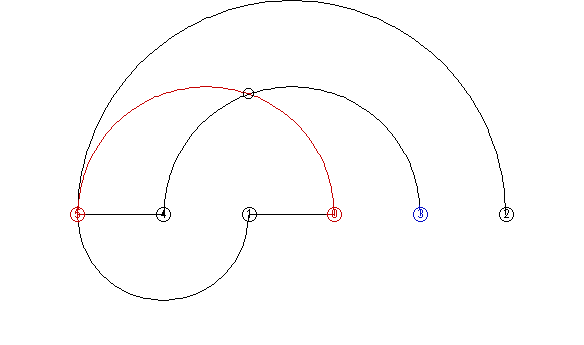
\includegraphics[width=0.33\textwidth]{imagenes/grafo_intercambio_original_bn.png}
			\label{subfig:ejemplo_mutacion_orig}
		}
		\subfigure[Grafo luego de intercambiar el nodo en la posición 0 por el de la posición 1.]{
			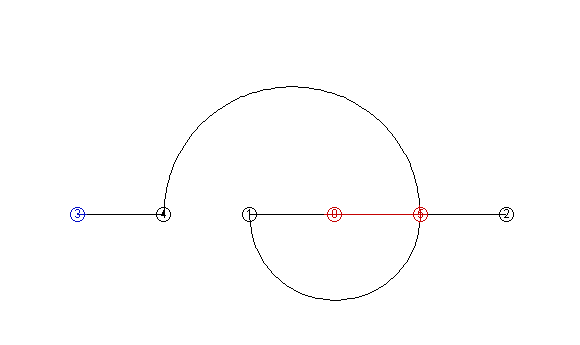
\includegraphics[width=0.33\textwidth]{imagenes/grafo_intercambio_nodo_bn.png}
			\label{subfig:ejemplo_mutacion_nodo}
		}
		\subfigure[Grafo luego de transponer el semiplano donde se grafica el arco entre los nodos en las posiciones 0 y 3.]{
			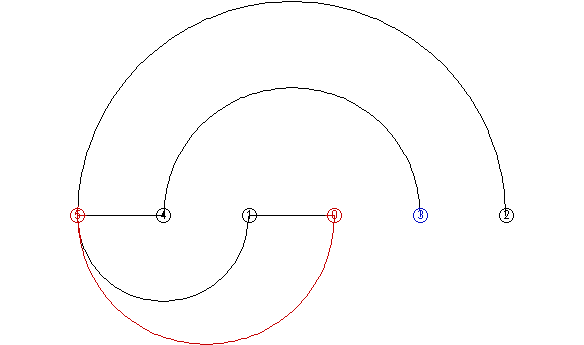
\includegraphics[width=0.33\textwidth]{imagenes/grafo_intercambio_arco_bn.png}
			\label{subfig:ejemplo_mutacion_arco}
		}
		\caption{Ejemplo de intercambio de nodos y cambio del semiplano donde se grafican los arcos.}
		\label{fig:ejemplo_mutacion}
	\end{figure*}
	
	%figura de ejemplo mostrando un intercambio de nodos y un cambio de sentido de arco.
	
	Por lo tanto, la cantidad de individuos de la población inicial está dada por la siguiente fórmula:
	
	$$num_{P_0} = m+V^2_n= m+ \frac{n!}{(n-2)!}=m+n^2-n $$siendo $m$ la cantidad de arcos del grafo y $n$ la cantidad de nodos.
	
	\subsection{Mutación}
	\label{subsec:mutacion}
	El algoritmo  genético propuesto utiliza   mutación en sus individuos, pero en esta primer versión  no se aplica crossover. Esta decisión de  diseño está basada en 
	algoritmos genéticos  con  objetivos similares \cite{he2007parallelisation, eloranta2001timga}. Sus autores especifican que  el crossover no es muy eficiente para resolver este problema, según los resultados experimentales obtenidos, por lo que se proponen porcentajes de mutación más altos y un crossover mínimo.
	%A partir del   relevamiento y análisis de algunos algoritmos genéticos  con  objetivos similares \cite{he2007parallelisation, eloranta2001timga}, en los cuáles se muestra que el crossover no es muy eficiente para este problema, según los resultados experimentales obtenidos, por lo que se proponen porcentajes de mutación más altos y un crossover mínimo.
	
	%En este sentido, para nuestro algoritmo se ha considerado anular el crossover y simplificar el problema a solo mutación. 
	Se proponen dos tipos de mutaciones posibles, con porcentajes basados en los utilizados en los trabajos \cite{he2007parallelisation, eloranta2001timga}:
	
	\begin{itemize}
		\item La primera mutación consiste en una transposición del  semiplano donde se grafica  un arco elegido al azar, como se muestra en la Figura \ref{subfig:ejemplo_mutacion_arco}. A está mutación se le ha dado un porcentaje de ocurrencia del 10\%.
		\item La segunda mutación consiste en el intercambio de orden de dos nodos elegidos al azar, como se muestra en la Figura \ref{subfig:ejemplo_mutacion_nodo}. A esta mutación se le ha dado un porcentaje de ocurrencia del 30\%.
	\end{itemize}
	
	Cada una de estas mutaciones,  son aplicadas a  cada individuo de la generación actual, buscando optimizar su Crossing Number.
	
	\subsection{Selección de Individuos}
	\label{subsec:seleccion_individuos}
	Una vez realizada la mutación del individuo se compara su Crossing Number (función de fitness) con el de la representación gráfica original del grafo y si aquel posee menos cruces se lo conserva y en caso contrario se lo descarta.
	%\todo[inline, color=orange]{GIULIANO VER}
	La  nueva población estará conformada por  individuos con un mejor layout que la  original del  grafo, aunque podría ser peor que el layout de su padre. Esto mantiene una población heterogénea.
	
	Por otra parte, nótese que por el criterio de selección de individuos la población varía su  tamaño,  de generación en generación. La población podría ser vacía si todos los hijos fueran peores que el layout original (semilla de la  población inicial),  dando así, un criterio extra para el  corte del  algoritmo.
	
	%A partir los individuos que se conserven se repite el proceso de mutación de la sección \ref{subsec:mutacion}.
	
	%\todo[inline,color=softred]{R: en respuesta a las dos anteriores. Si, la población es variable, en cada generación, cada individuo se compara con el original y si no lo mejora es eliminado de la población. Esto puede provocar que se extinga la población. Por lo que se guarda el mejor individuo que mejore al original y este es el que es retornado (o el original si ninguno lo mejoró).}
	
	\subsection{Criterio de Finalización del Algoritmo }
	%Se ha propuesto realizar varios ciclos (no son generaciones) del algoritmo genético para determinar su corte. Esto es,
	Dada la población inicial, primer generación, gestada  a partir de su Diagrama de Arcos, como se describe  en la sección \ref{subsec:generar_poblacion_inicial}, se realizan $1000$ generaciones en las cuáles tales individuos se mutan. Los individuos nuevos pueden ser eliminados de la  población, en caso de no superar el Crossing Number de la representación gráfica original del grafo.
	
	Una vez finalizadas las generaciones o extinta la población, se retorna el mejor Diagrama de Arcos obtenido y se comienza un nuevo ciclo utilizando este último como semilla generadora de la población inicial. Esto se repite hasta alcanzar un número máximo de ciclos  o cuando se iguala el número de cruces de  la mejor representación gráfica obtenida en dos ciclos consecutivos.
	
	%Un ciclo termina si se obtiene un Diagrama de Arcos sin cruces de arcos, o si se cumple con un número determinado de generaciones, o si la población se extingue, es decir ya no quedan individuos. En cualquiera de los casos se devolverá el mejor grafo obtenido o en caso de no mejorar el resultado, el mismo que se envío como entrada.
	
	%Mutación:
	%\begin{itemize}
	%    \item Intercambio de arco: arriba-abajo (10\%)
	%    \item Intercambio nodo al azar (30\%)
	%\end{itemize}
	
	%Argumentar  sobre los  porcentajes con el paper de paralelización
	
	%Cada  generación tiene una cantidad de $$m+V^2_n= m+ \frac{n!}{(n-2)!}=m+n^2-n $$ siendo  m cantidad de arcos y n cantidad de nodos
	
	%Los nodos con grado más alto probablemente sea  el centro del grafo. Si hubiera  más de un nodo  con alto grado  se deberán balancear.\\
	
	%Explicar la heurística: nro de cruces. 
	
	%Ejemplificar

\section{Integración con Algoritmos de Layout para Grafos Genéricos}
